\documentclass[10pt]{article}

\usepackage{mathtools, amsfonts, bm}
\usepackage{microtype}
\usepackage[utf8]{inputenc}
\usepackage[top = 1.0in, left = 1.75in, right = 0.75in, bottom = 0.75in]{geometry}
\usepackage{booktabs}
\usepackage{graphicx}
\usepackage{xcolor}
\usepackage{tabularx}
\usepackage{tikzsymbols}
\usepackage[hidelinks]{hyperref}

\usepackage[explicit]{titlesec}
\titleformat{\section}[runin]{\bfseries}{}{0em}{
    \llap{
        \smash{
            \begin{tabularx}{0.75in}[t]{@{}l@{\hskip0.4em}>{\raggedright}X@{\hskip\marginparsep}}
                #1 
            \end{tabularx}
        }
    }
}[\leavevmode\hspace*{\dimexpr-\fontdimen2\font-\fontdimen3\font+0.375em}]

\usepackage{fancyhdr}
\pagestyle{fancy}
\fancyhf{}
\rhead{\thepage}
\renewcommand{\headrulewidth}{0pt}

\usepackage{lipsum}

%' ============================================================================================================================================================
%' ============================================================================================================================================================

\begin{document}

\newcommand{\mytitle}{Homework 1}
\newcommand{\myauthor}{Aiden Kenny}
\newcommand{\myclass}{STAT GR5205: Linear Regression Models}
\newcommand{\myschool}{Columbia Univeristy}
\newcommand{\mydate}{September 21, 2020}
\begin{flushright}
    \textbf{\mytitle}\\[0.5em]
    \textsl{\myauthor}\\
    \textsl{\myclass}\\
    \textsl{\myschool}\\
    \textsl{\mydate}
\end{flushright} \vspace{1em}

%' ============================================================================================================================================================
\section{Question 1} \noindent
% We will first read in the data using the \verb|data.table| package, and we will make our
% plots using the \verb|ggplot2| package.
% \begin{verbatim}
% library(data.table)
% library(ggplot2)
% cm <- fread(input = 'data/copier_maintenance.txt')
% \end{verbatim}
\begin{figure}[ht]
    \centering
    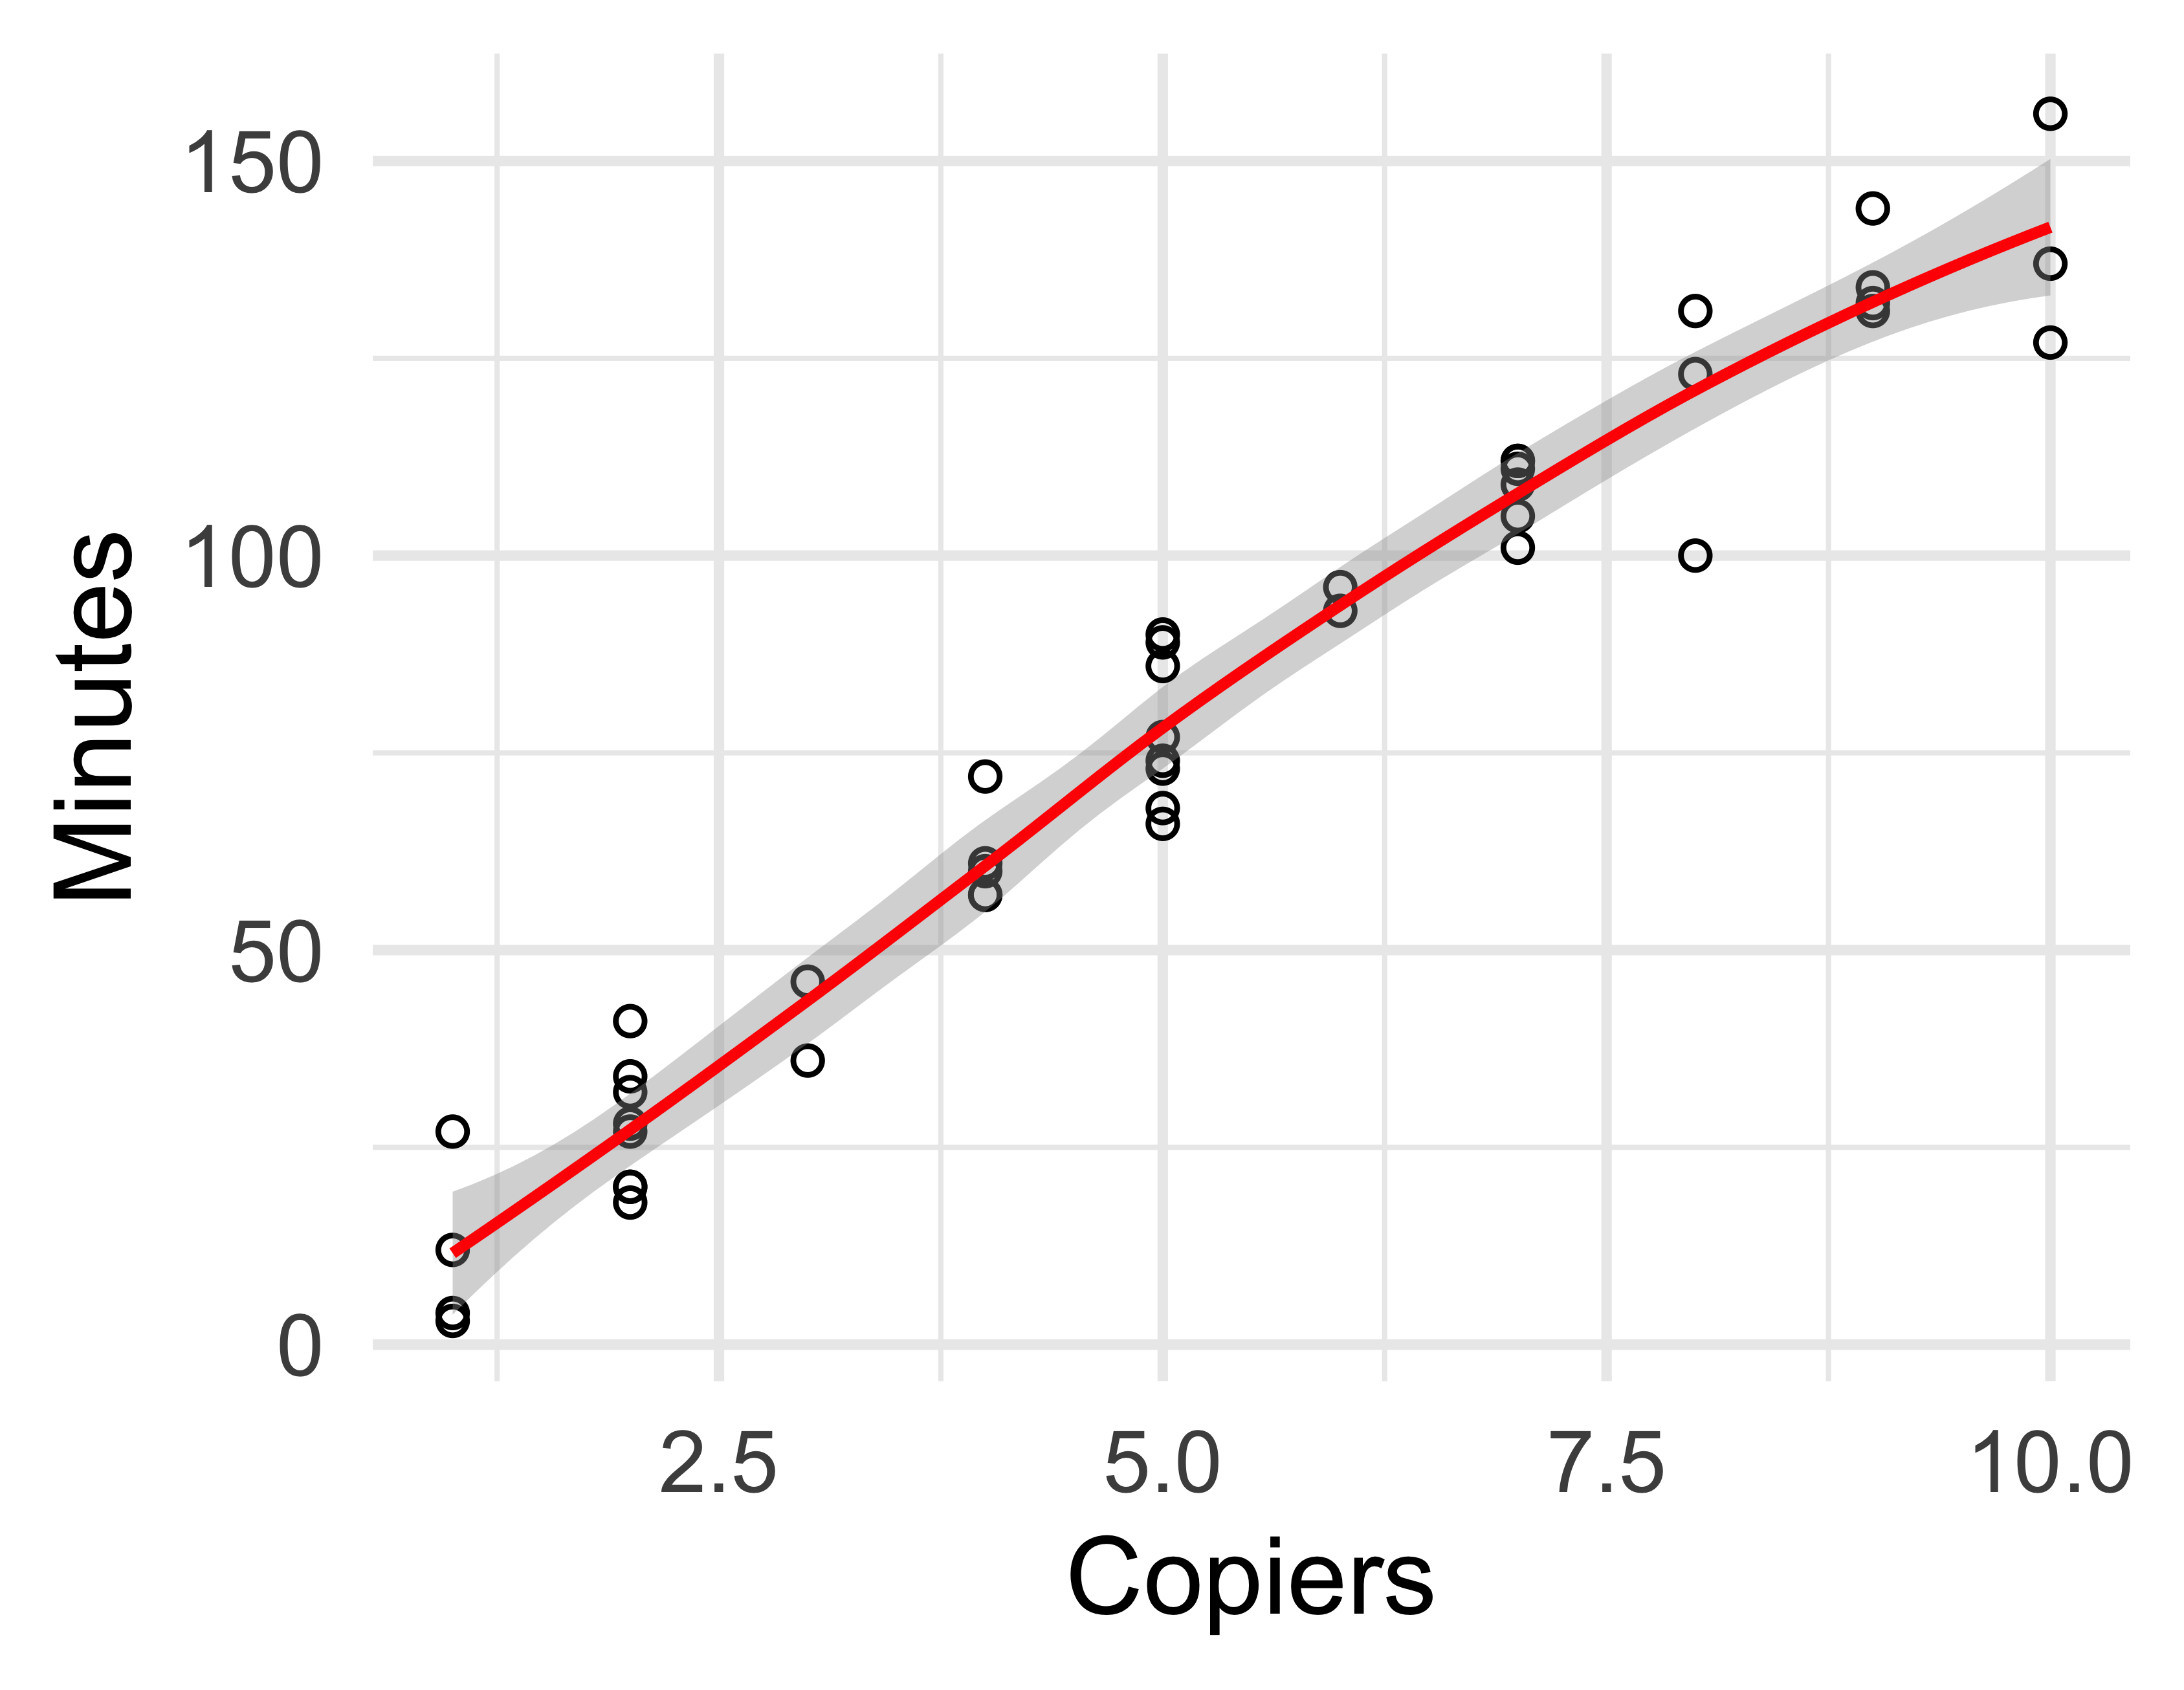
\includegraphics[width = 0.45\textwidth]{q01_lowess.png}
    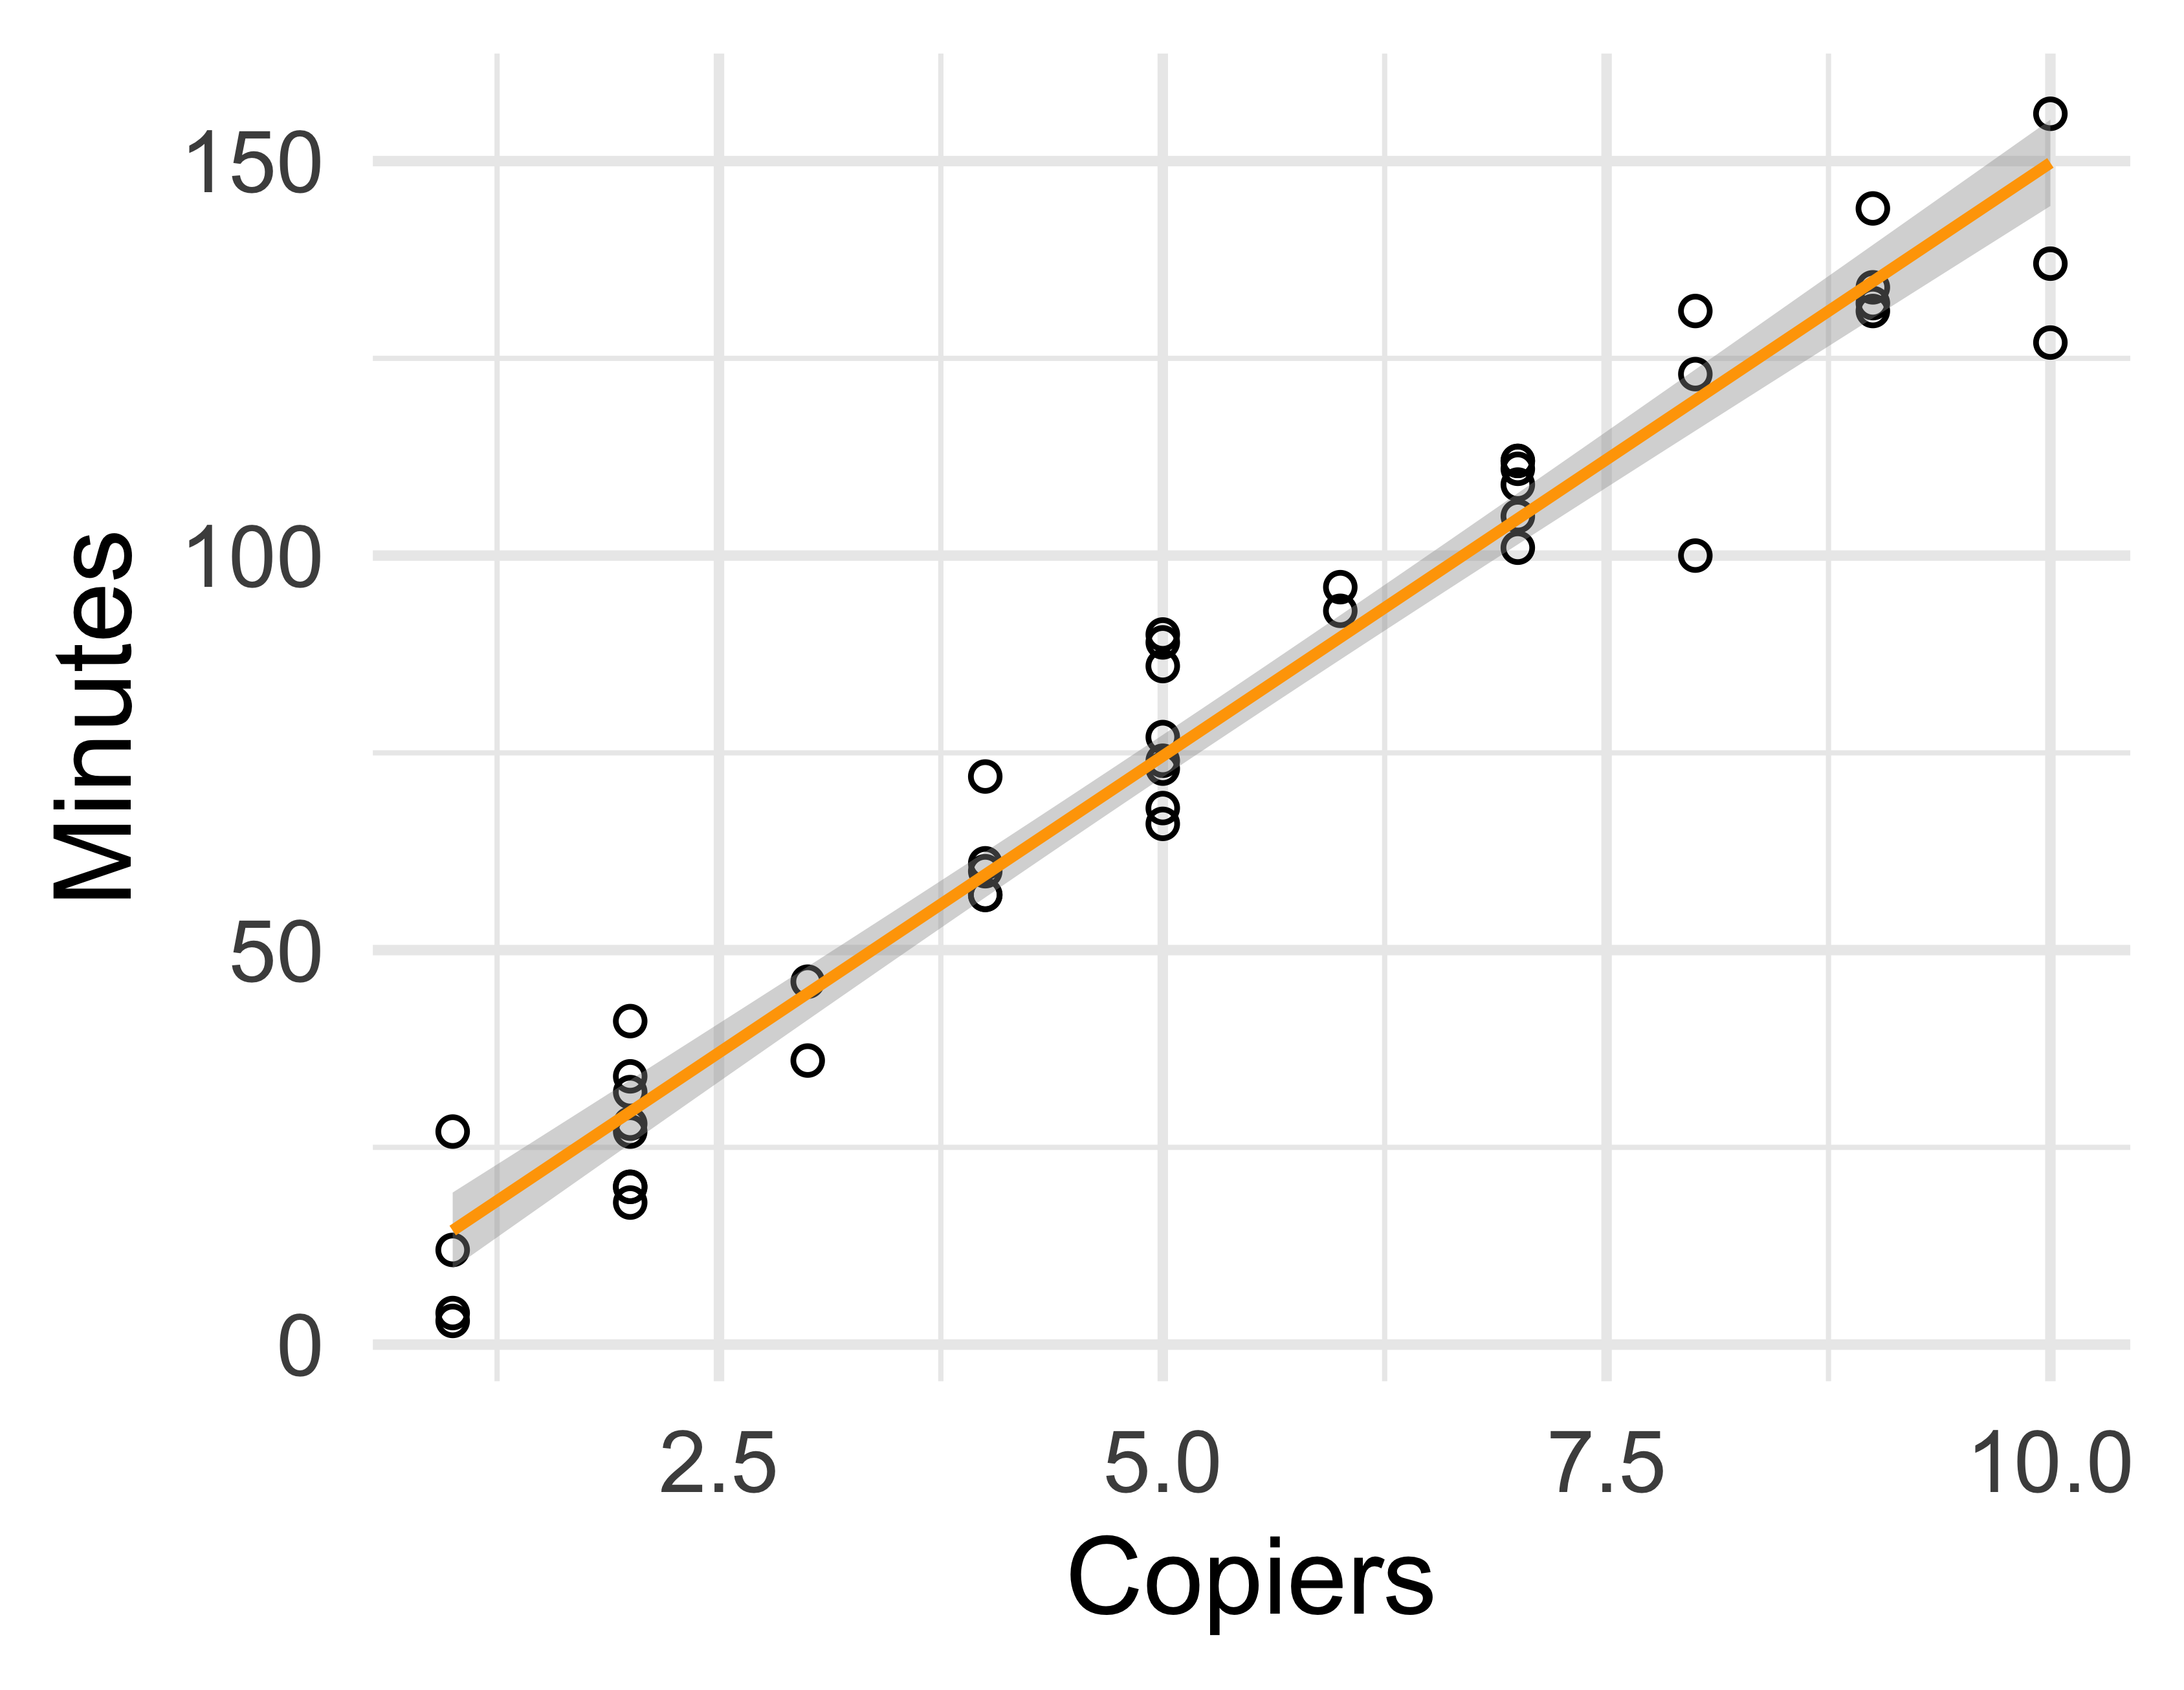
\includegraphics[width = 0.45\textwidth]{q01_linear.png}
    \caption{Left: overlaying a loess smoother to a scatterplot of the data. Right: 
    overlaying the estimated linear regression model to the scatterplot.}
    \label{q01_fig}
\end{figure} 
\begin{itemize}
    \item[(a)] The loess smoother has been overlayed the data in the left panel of Figure \ref{q01_fig}. Here we 
    can see that the line is essentailly a straight line, implying that the true relationship is linear. 
    \item[(b)] Using \texttt{R}, our estimated coefficients are given by \(b_0 = -0.5801567\)
    and \(b_1 = 15.0352480\), and so our estimated linear regression function is given by
    \[\hat{Y} = -0.5801567 + 15.0352480 X.\] The estimated linear regression model has been 
    overlayed on a scatterplot of the data in the right plot in Figure \ref{q01_fig}, and the 
    estimated function seems to fit the data well. The general trend, where an increase in number of 
    copiers results in an increased number of minutes on call, is captured by the model.
    \item[(c)] \(b_1\) can be interpreted as follows. If the number of copiers serviced during
    a call increased by one, the total number of minutes of the call is expected to \textit{increase} by 
    \(15.0352480\) minutes. 
    \item[(d)] \(b_0\) can be interpreted as follows. If there are zero copiers serviced during 
    a call, then we can expect the call to last for, on average, \(-0.5801567 \) minutes. This does \textit{not}
    provide any useful or relevant information; a call cannot ever have negative time, and a customer would never
    call if they did not have any copiers to service (where \(X = 0\)).
    \item[(e)] When there are five copiers (\(X=5\)), a point estimate for the mean service time is 
    \[
        \hat{Y}(5) = -0.5801567 + 15.0352480(5) = 74.59608.
    \]
    \item[(f)] A point \textit{prediction} for minutes when \(X=5\) would \textit{also} be \(\hat{Y} = 74.59608\). Note that
    even though the two values are numerically identical, they have different meanings. 
    \item[(g)] Using \texttt{R}, we can see that the residuals sum to 0; this is easy to do since the residuals are
    are included in the fitted model. We can think of \(Q\) as a \textit{function} 
    of \(\beta_0\) and \(\beta_1\), and we want to find the values of \(\beta_0\) and \(\beta_1\) that minimize \(Q\).
    The observed residuals \(e_i\), when plugged into \(Q\), give the smallest value of \(Q\) that can possibly be obtained. 
    Let \(\bm{\varepsilon} = (\varepsilon_1, \ldots, \varepsilon_n)^T\) be the random vector containing the \(n\) 
    residuals, and let \(\mathbf{e} = (e_1, \ldots, e_n)^T\) be the \(n\) realized residuals from \(b_0\)
    and \(b_1\). Using this 
    notation, we have \(Q = \| \bm{\varepsilon} \|^2\), and \[\| \mathbf{e}\|^2 = \min \|\bm{\varepsilon}\|^2 = \min Q.\]
    \item[(h)] Using \texttt{R}, we can get a point estimate for \(\sigma^2\) as \(\hat{\sigma}^2 = \frac{1}{n-2} \|\mathbf{e}\|^2 = 79.45063\); note that we 
    \textit{are not} using the sample variance formula. A corresponding point estimate for \(\sigma\) is \(\hat{\sigma} = \sqrt{\hat{\sigma}^2} = 8.913508\). 
    \(\hat{\sigma}\) is expressed in the same units as \(Y\): minutes. 

\end{itemize}

%' ============================================================================================================================================================
\section{Question 2} \noindent
For this question, let \texttt{Stay} denote a patient's average stay in the hospital, \texttt{Risk} denote a patient's risk of infection, \texttt{AFS} 
denote the hospital's available facilities and services, and \texttt{Xray} denote a patient's routine chest X-ray ratio. 
\begin{figure}[ht]
    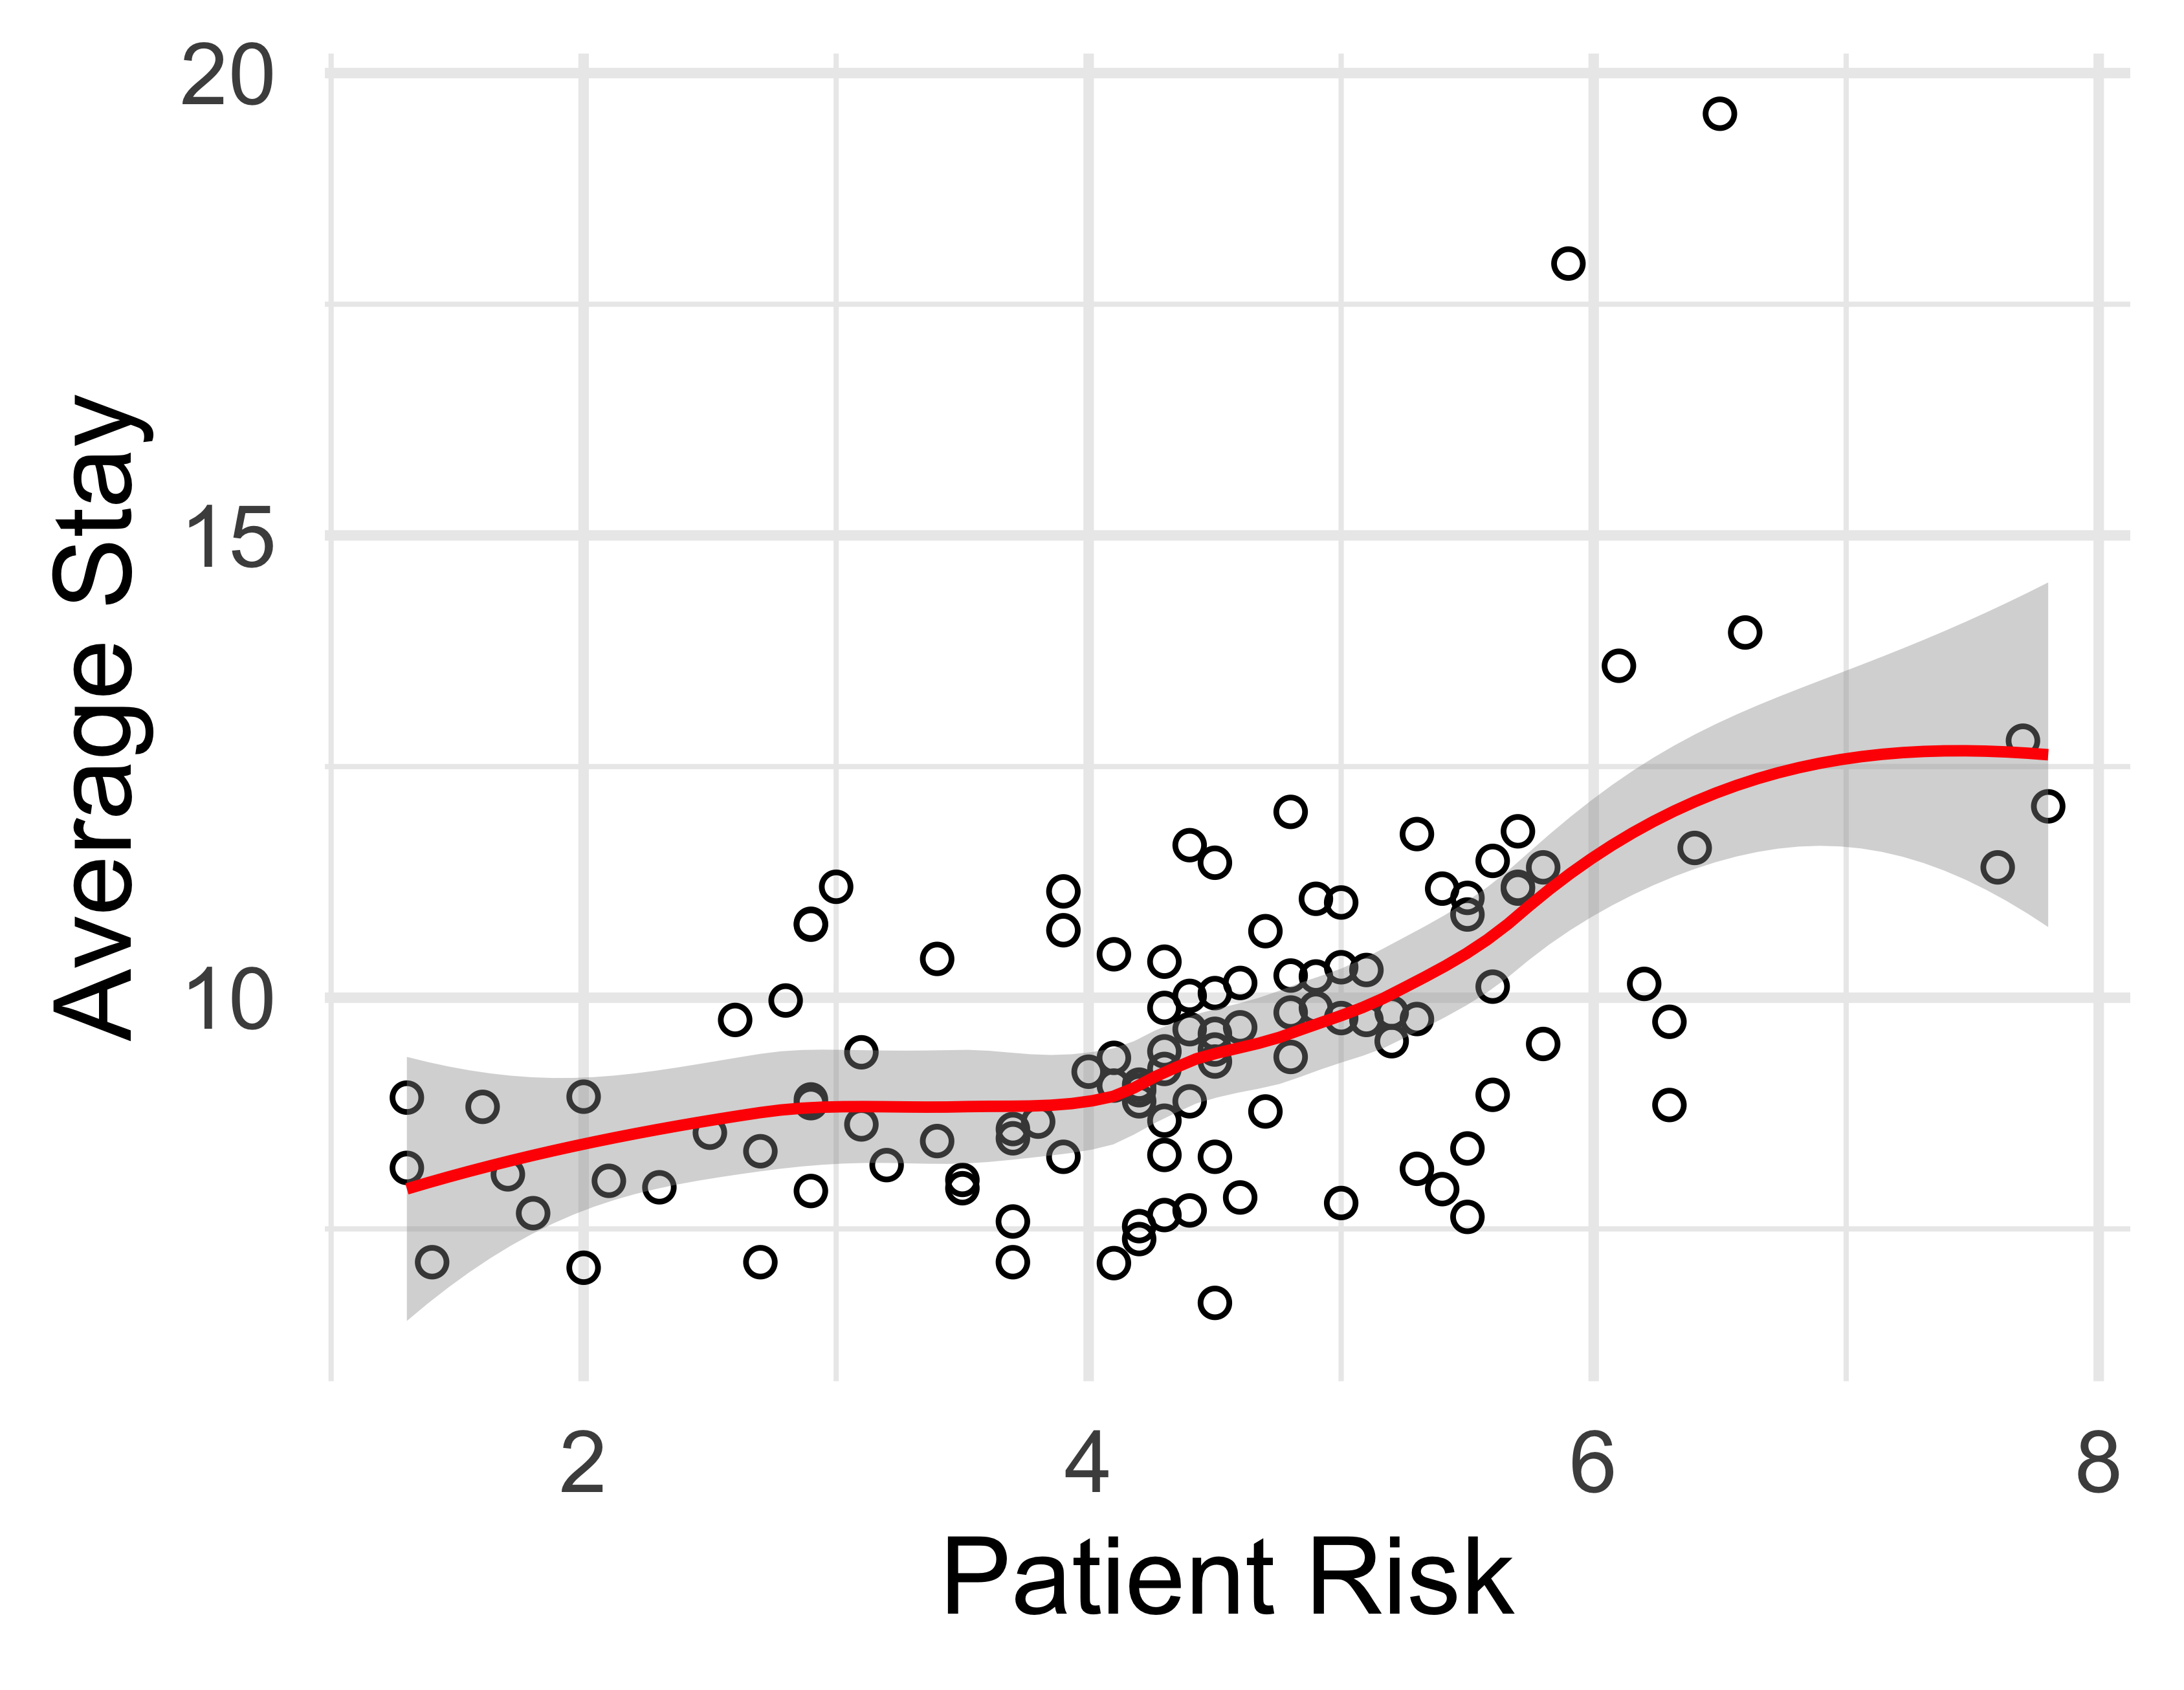
\includegraphics[width = 0.32\textwidth]{q02_loess1.png}
    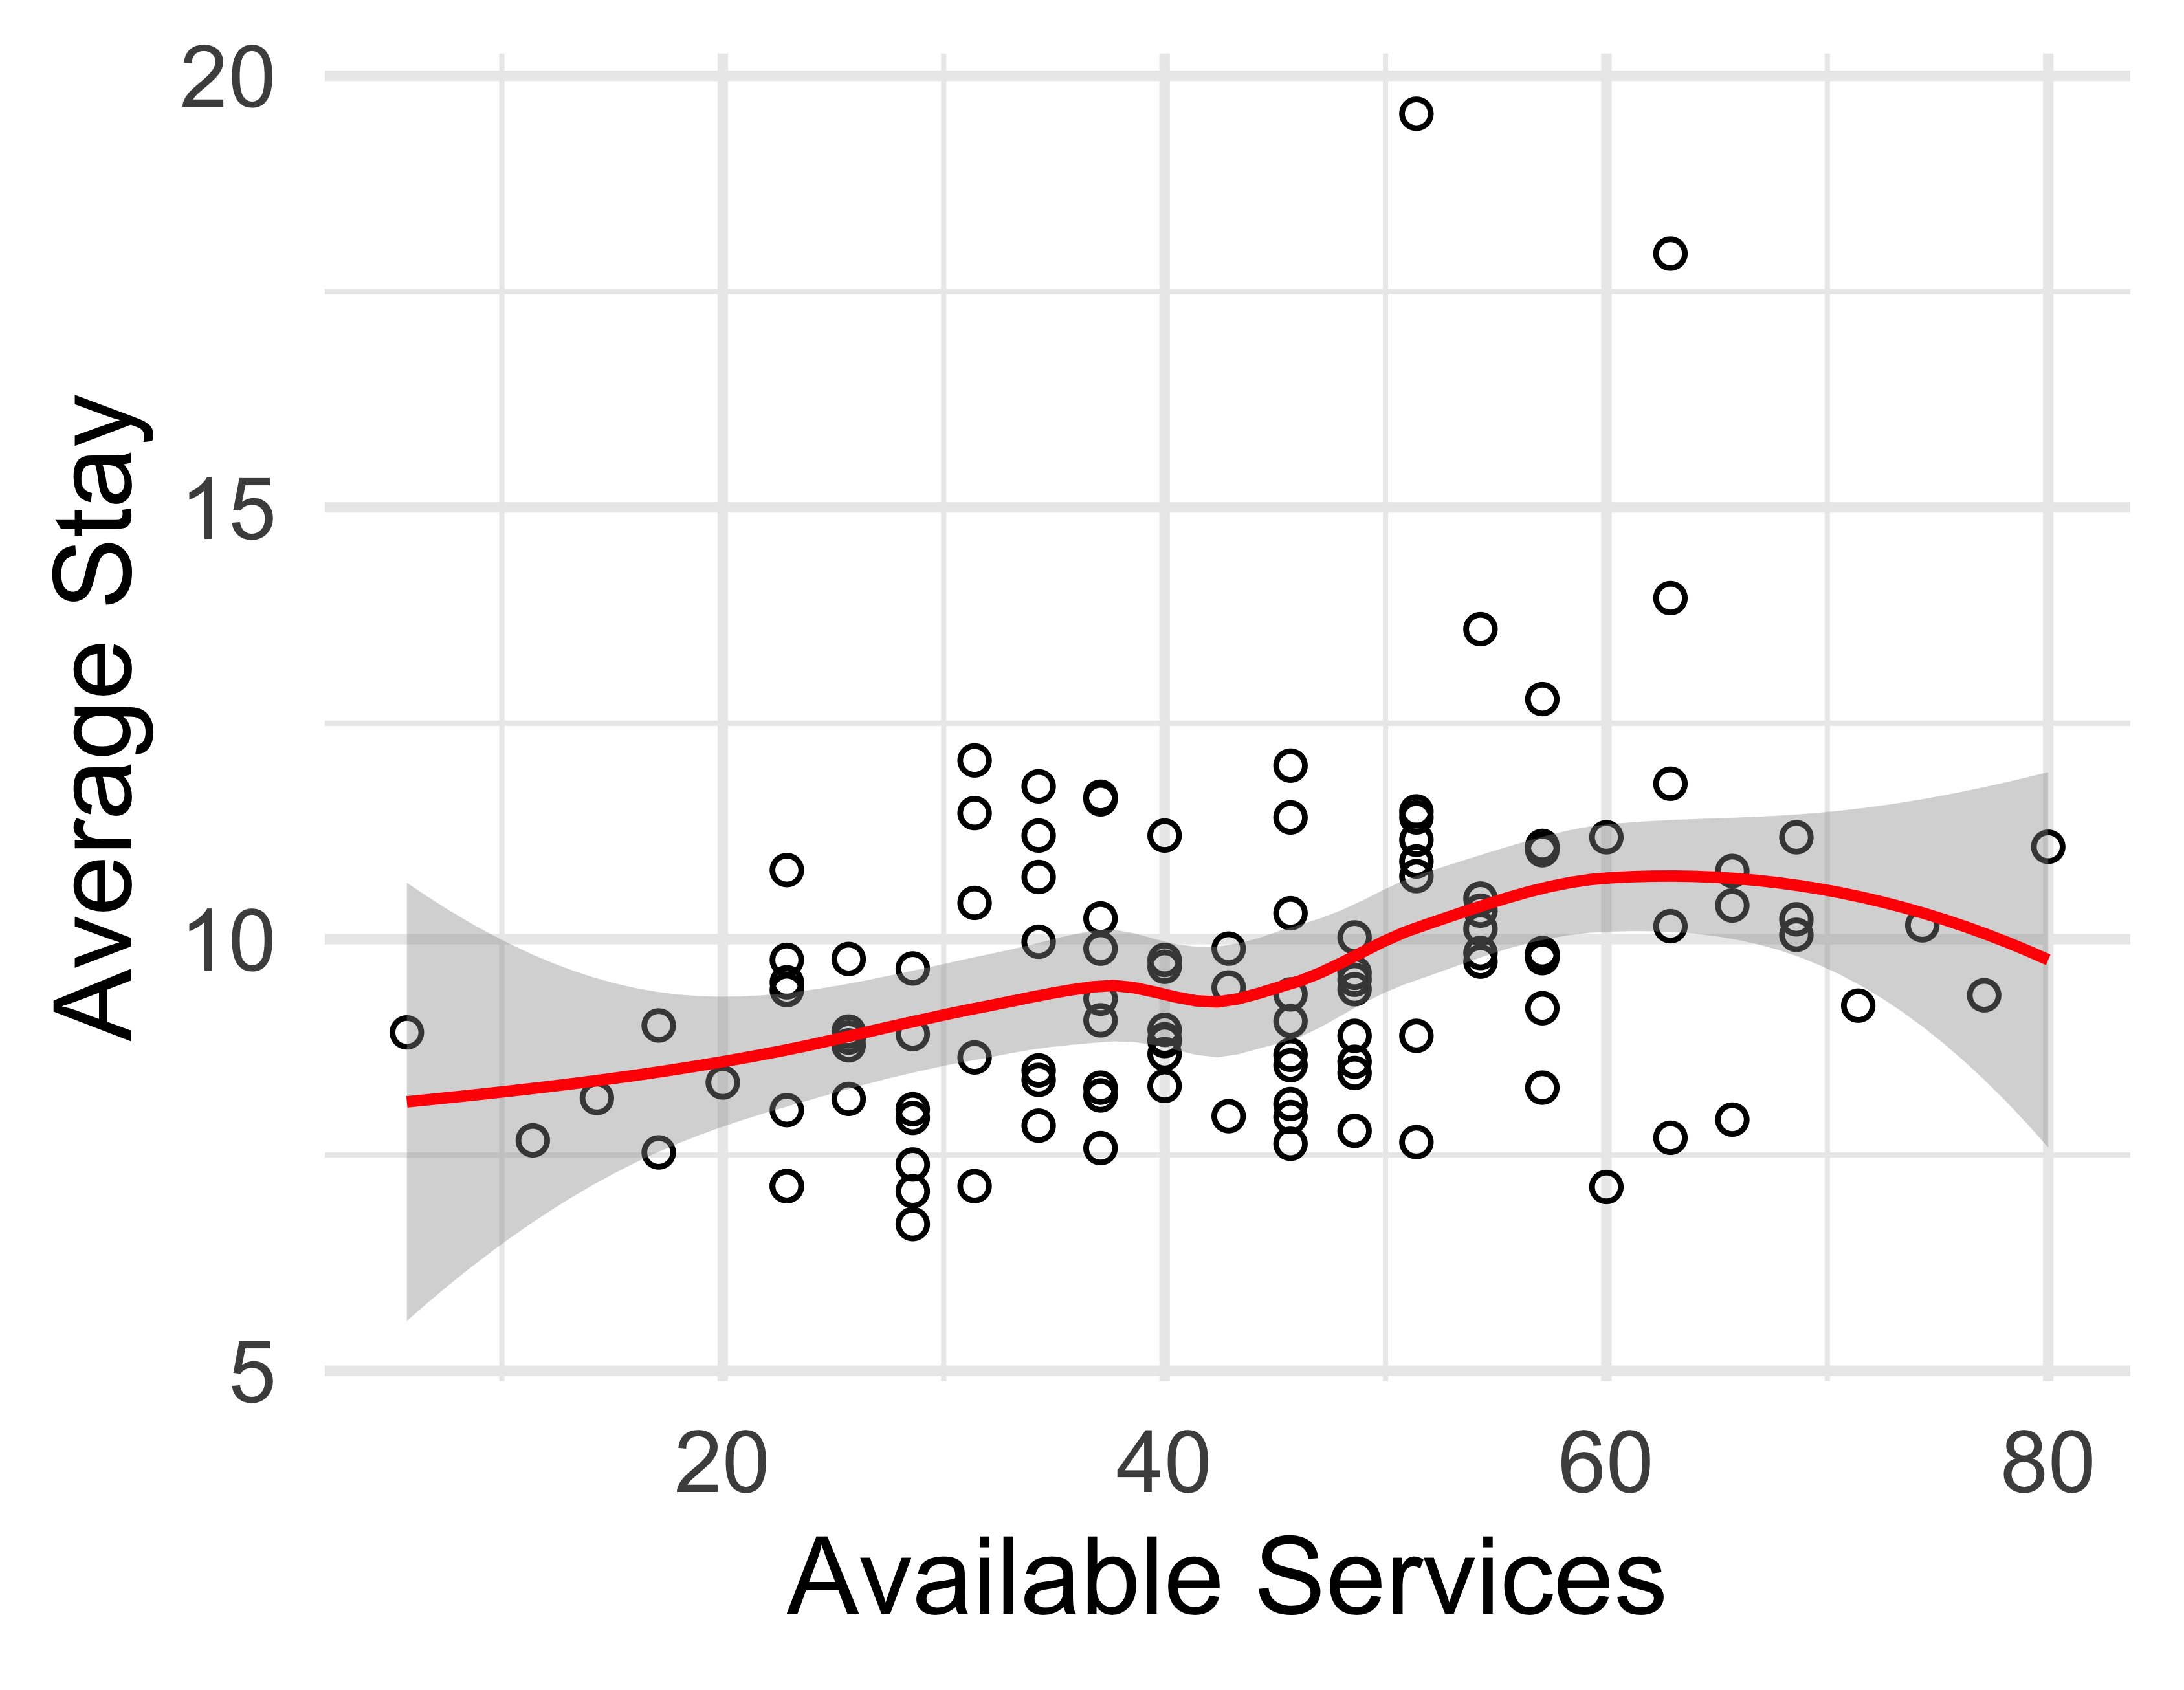
\includegraphics[width = 0.32\textwidth]{q02_loess2.png}
    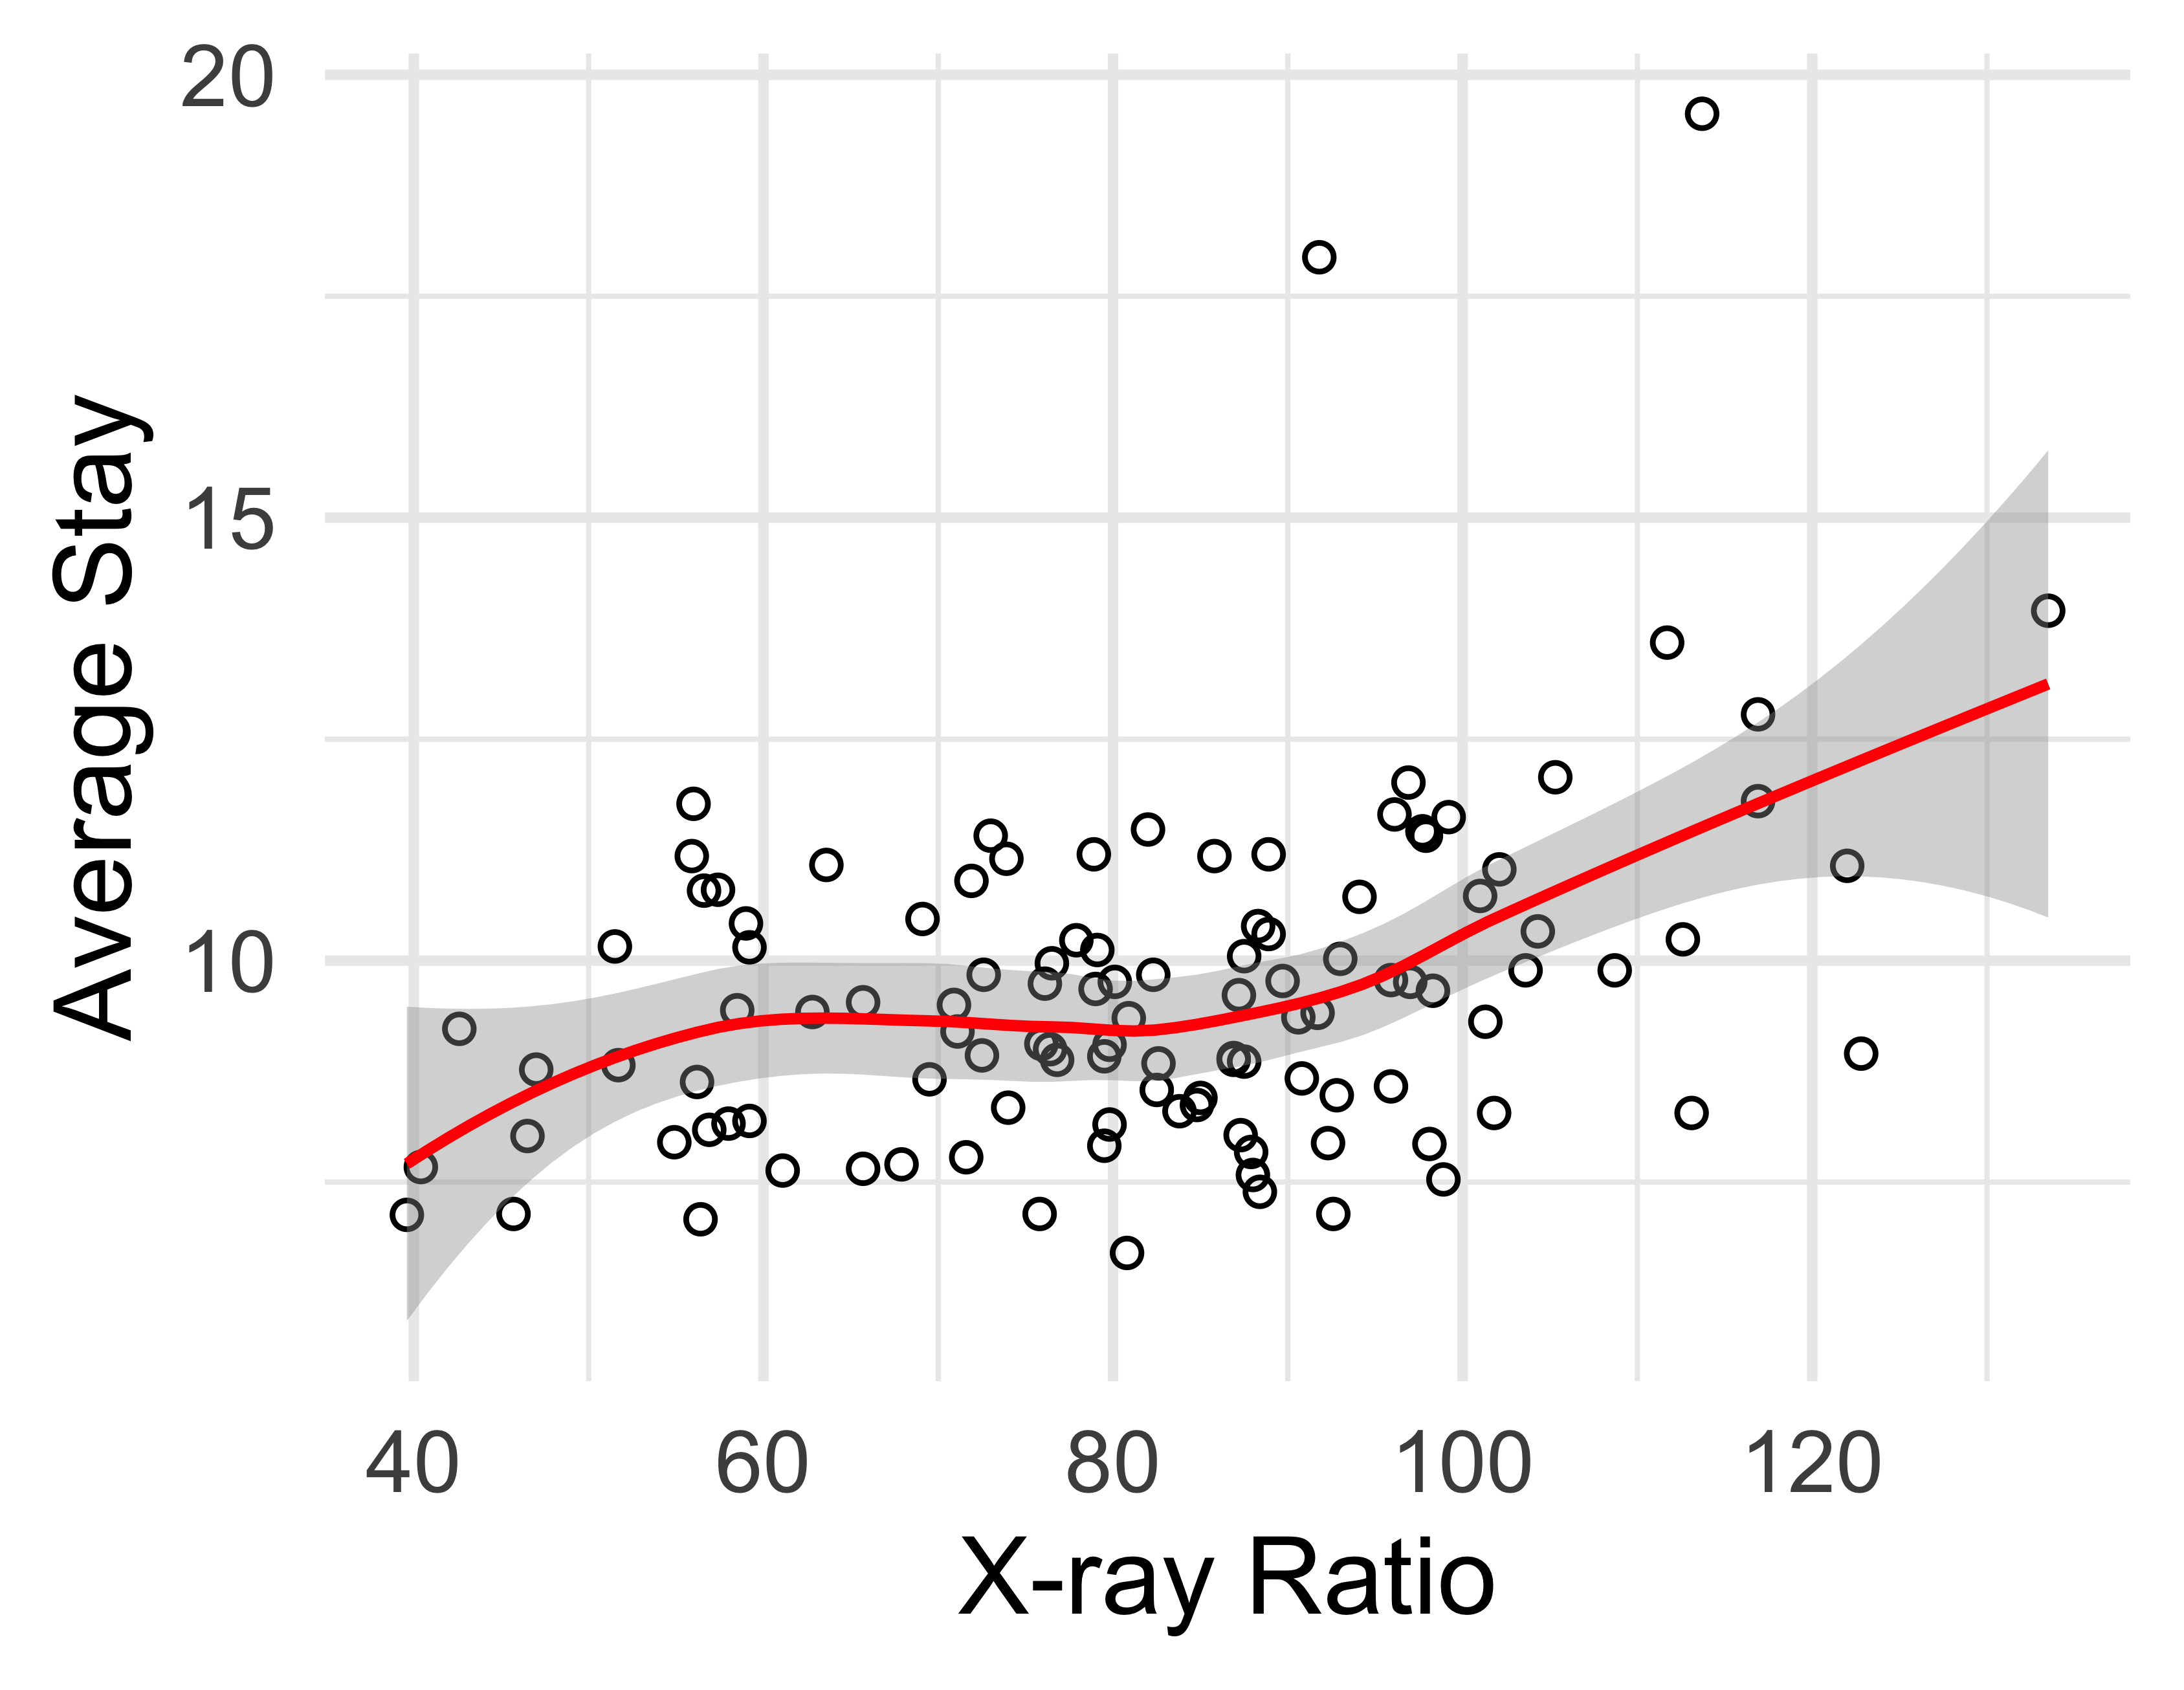
\includegraphics[width = 0.32\textwidth]{q02_loess3.png}
    \caption{Applying loess smoothers to the scatterplots of \texttt{Stay} against the three predictor variables: \texttt{Risk}, \texttt{AFS}, and 
    \texttt{Xray}.}
    \label{q02_fig01}
\end{figure}

\begin{figure}[ht]
    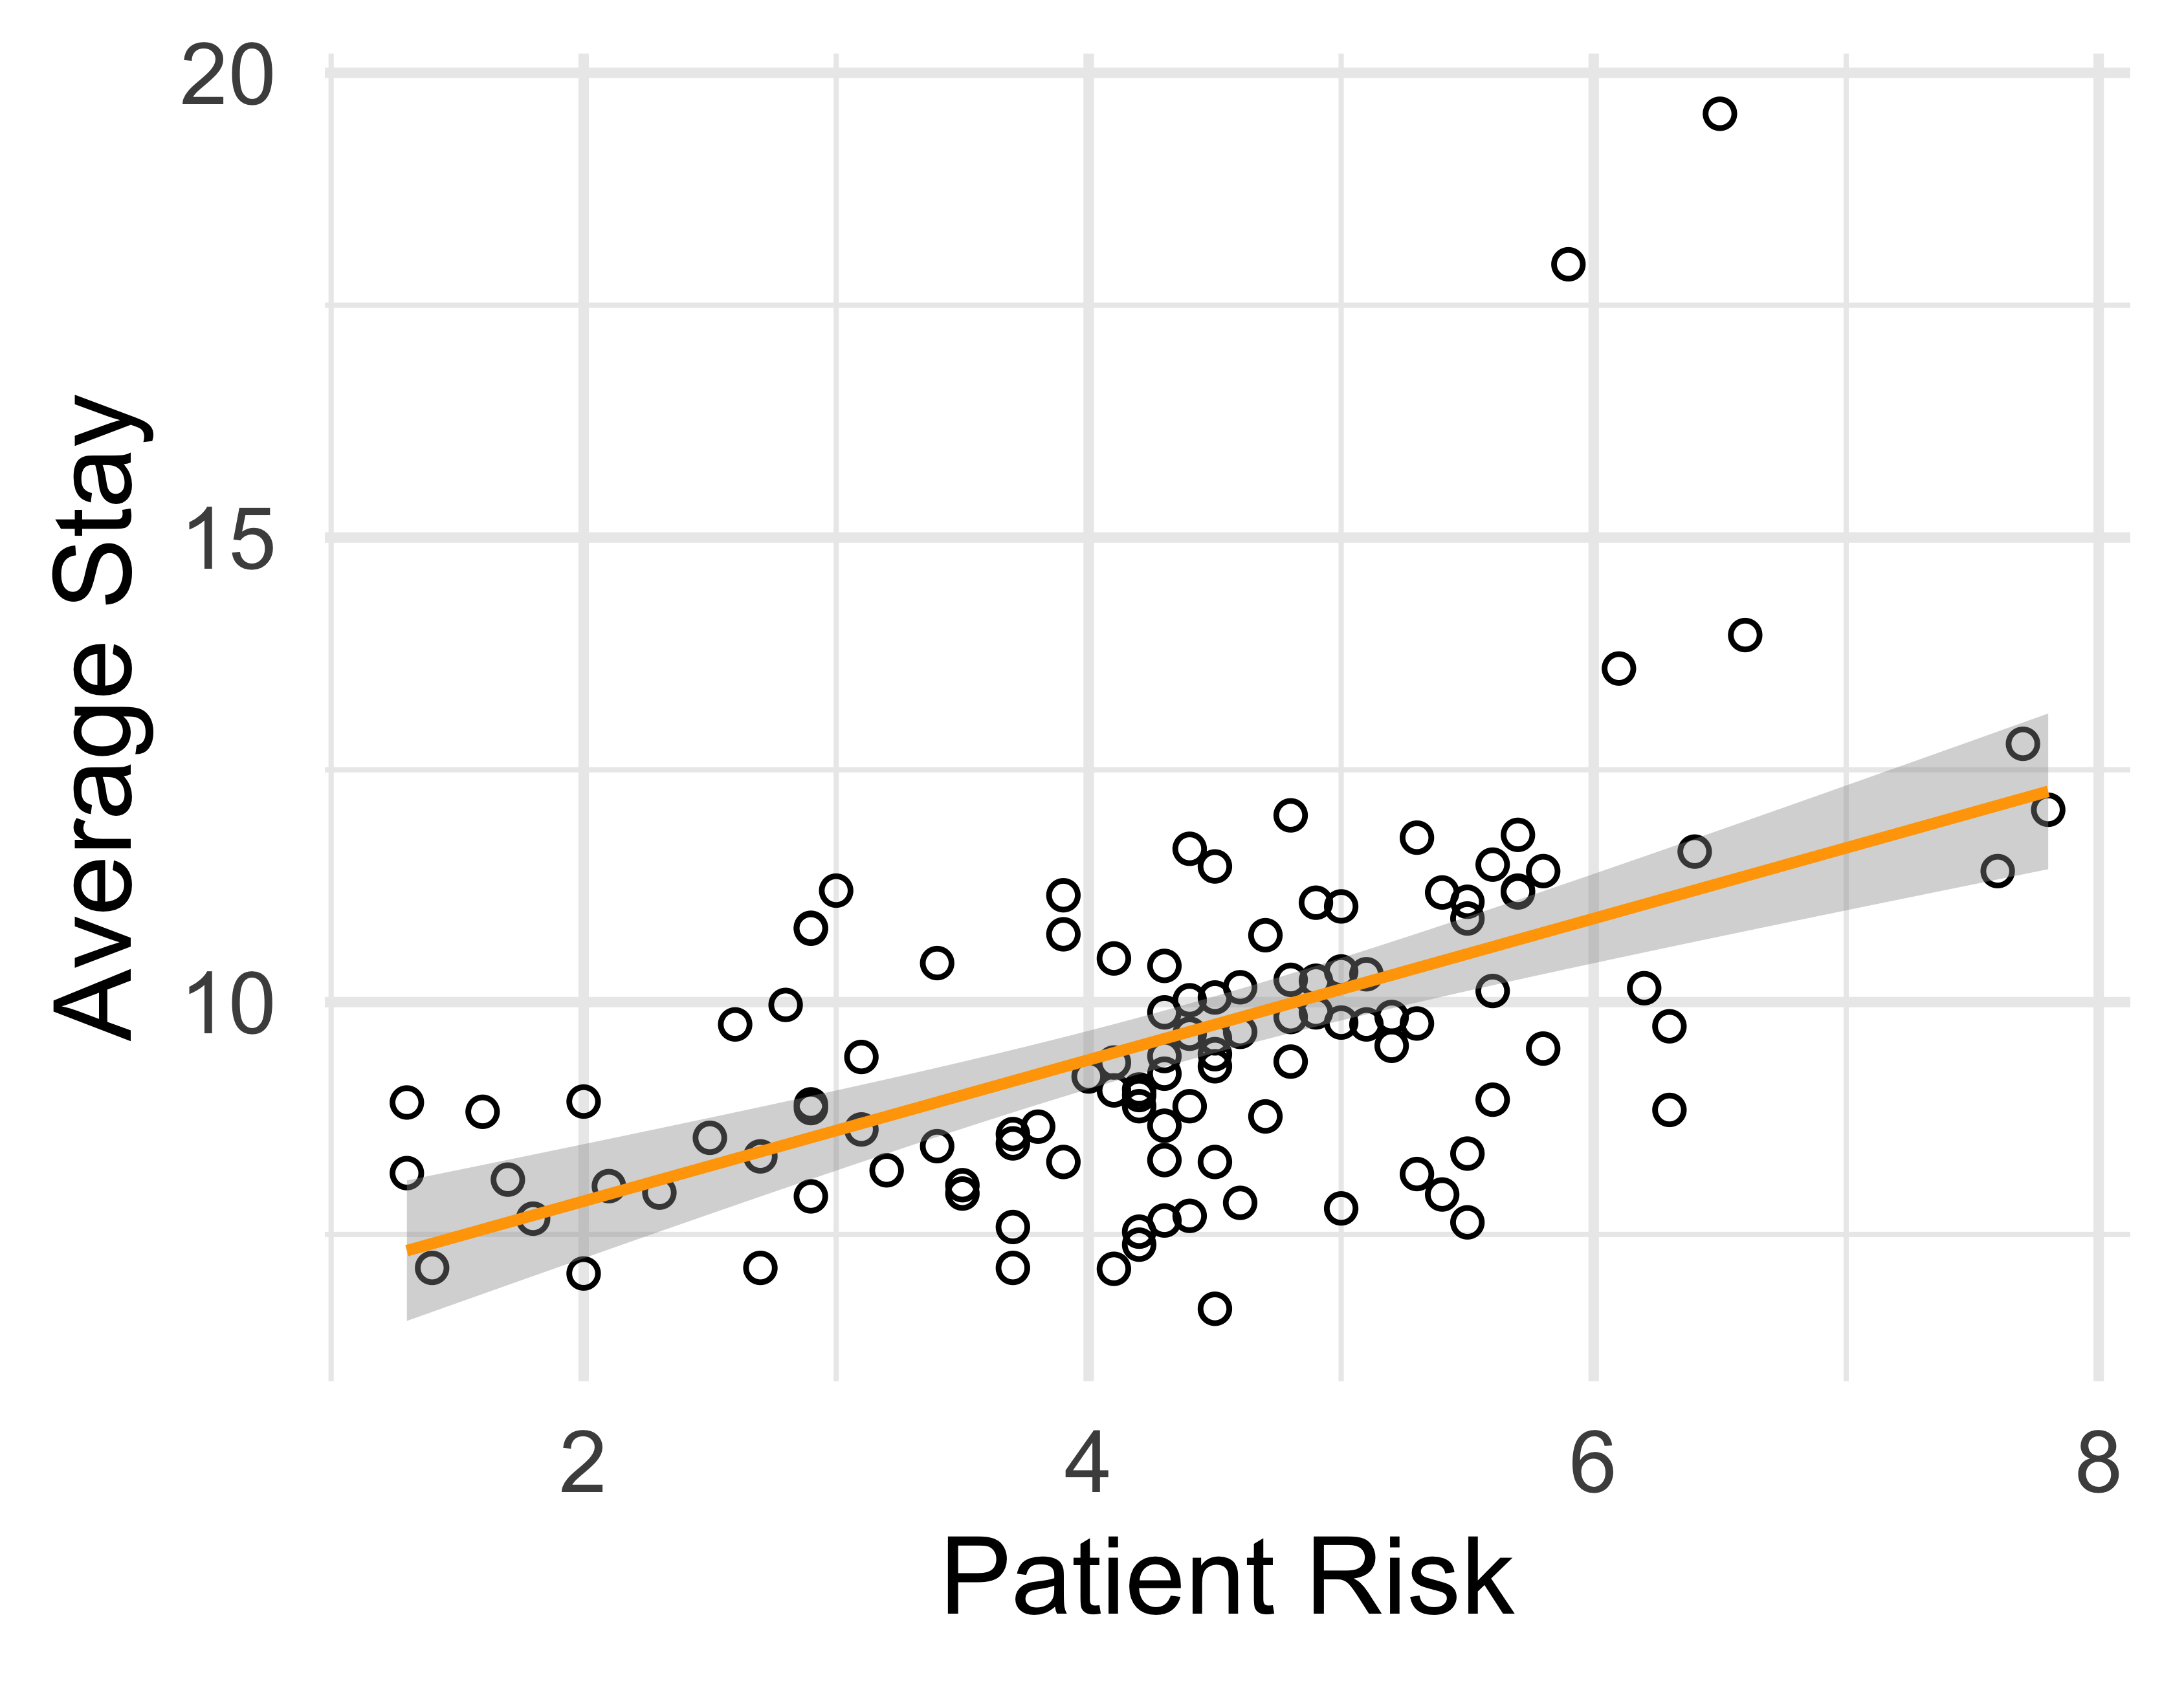
\includegraphics[width = 0.32\textwidth]{q02_lm1.png}
    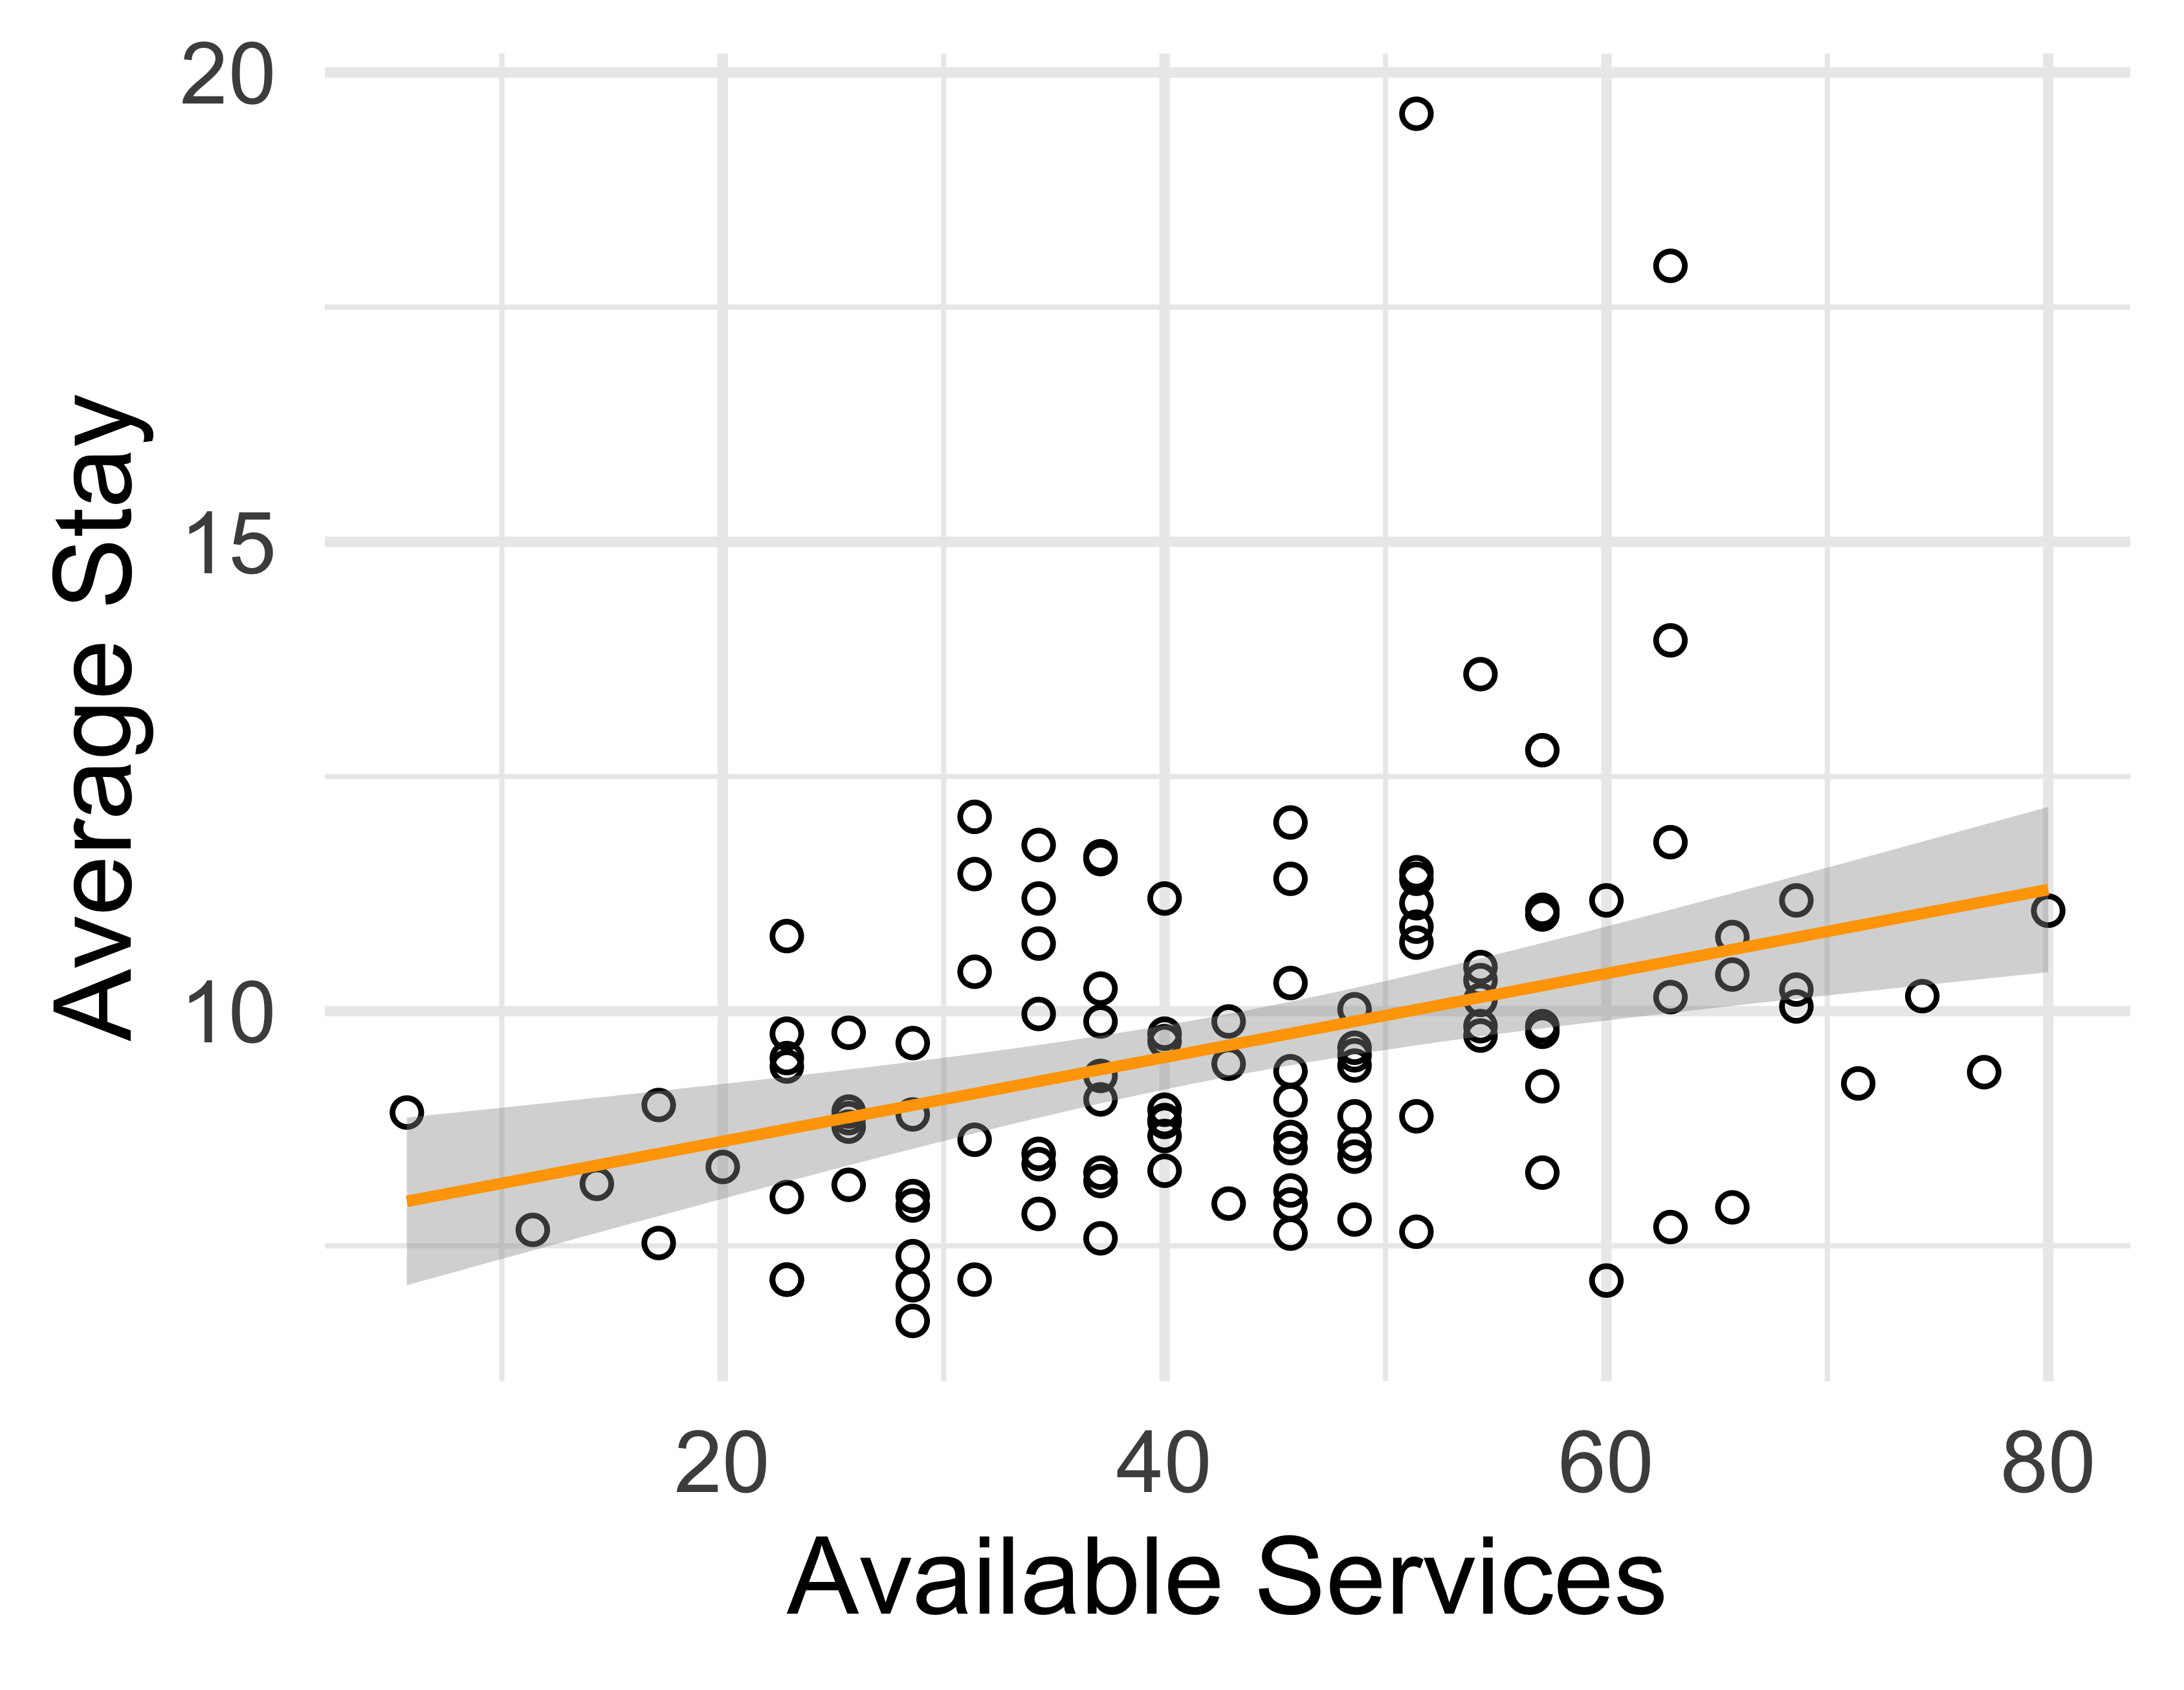
\includegraphics[width = 0.32\textwidth]{q02_lm2.png}
    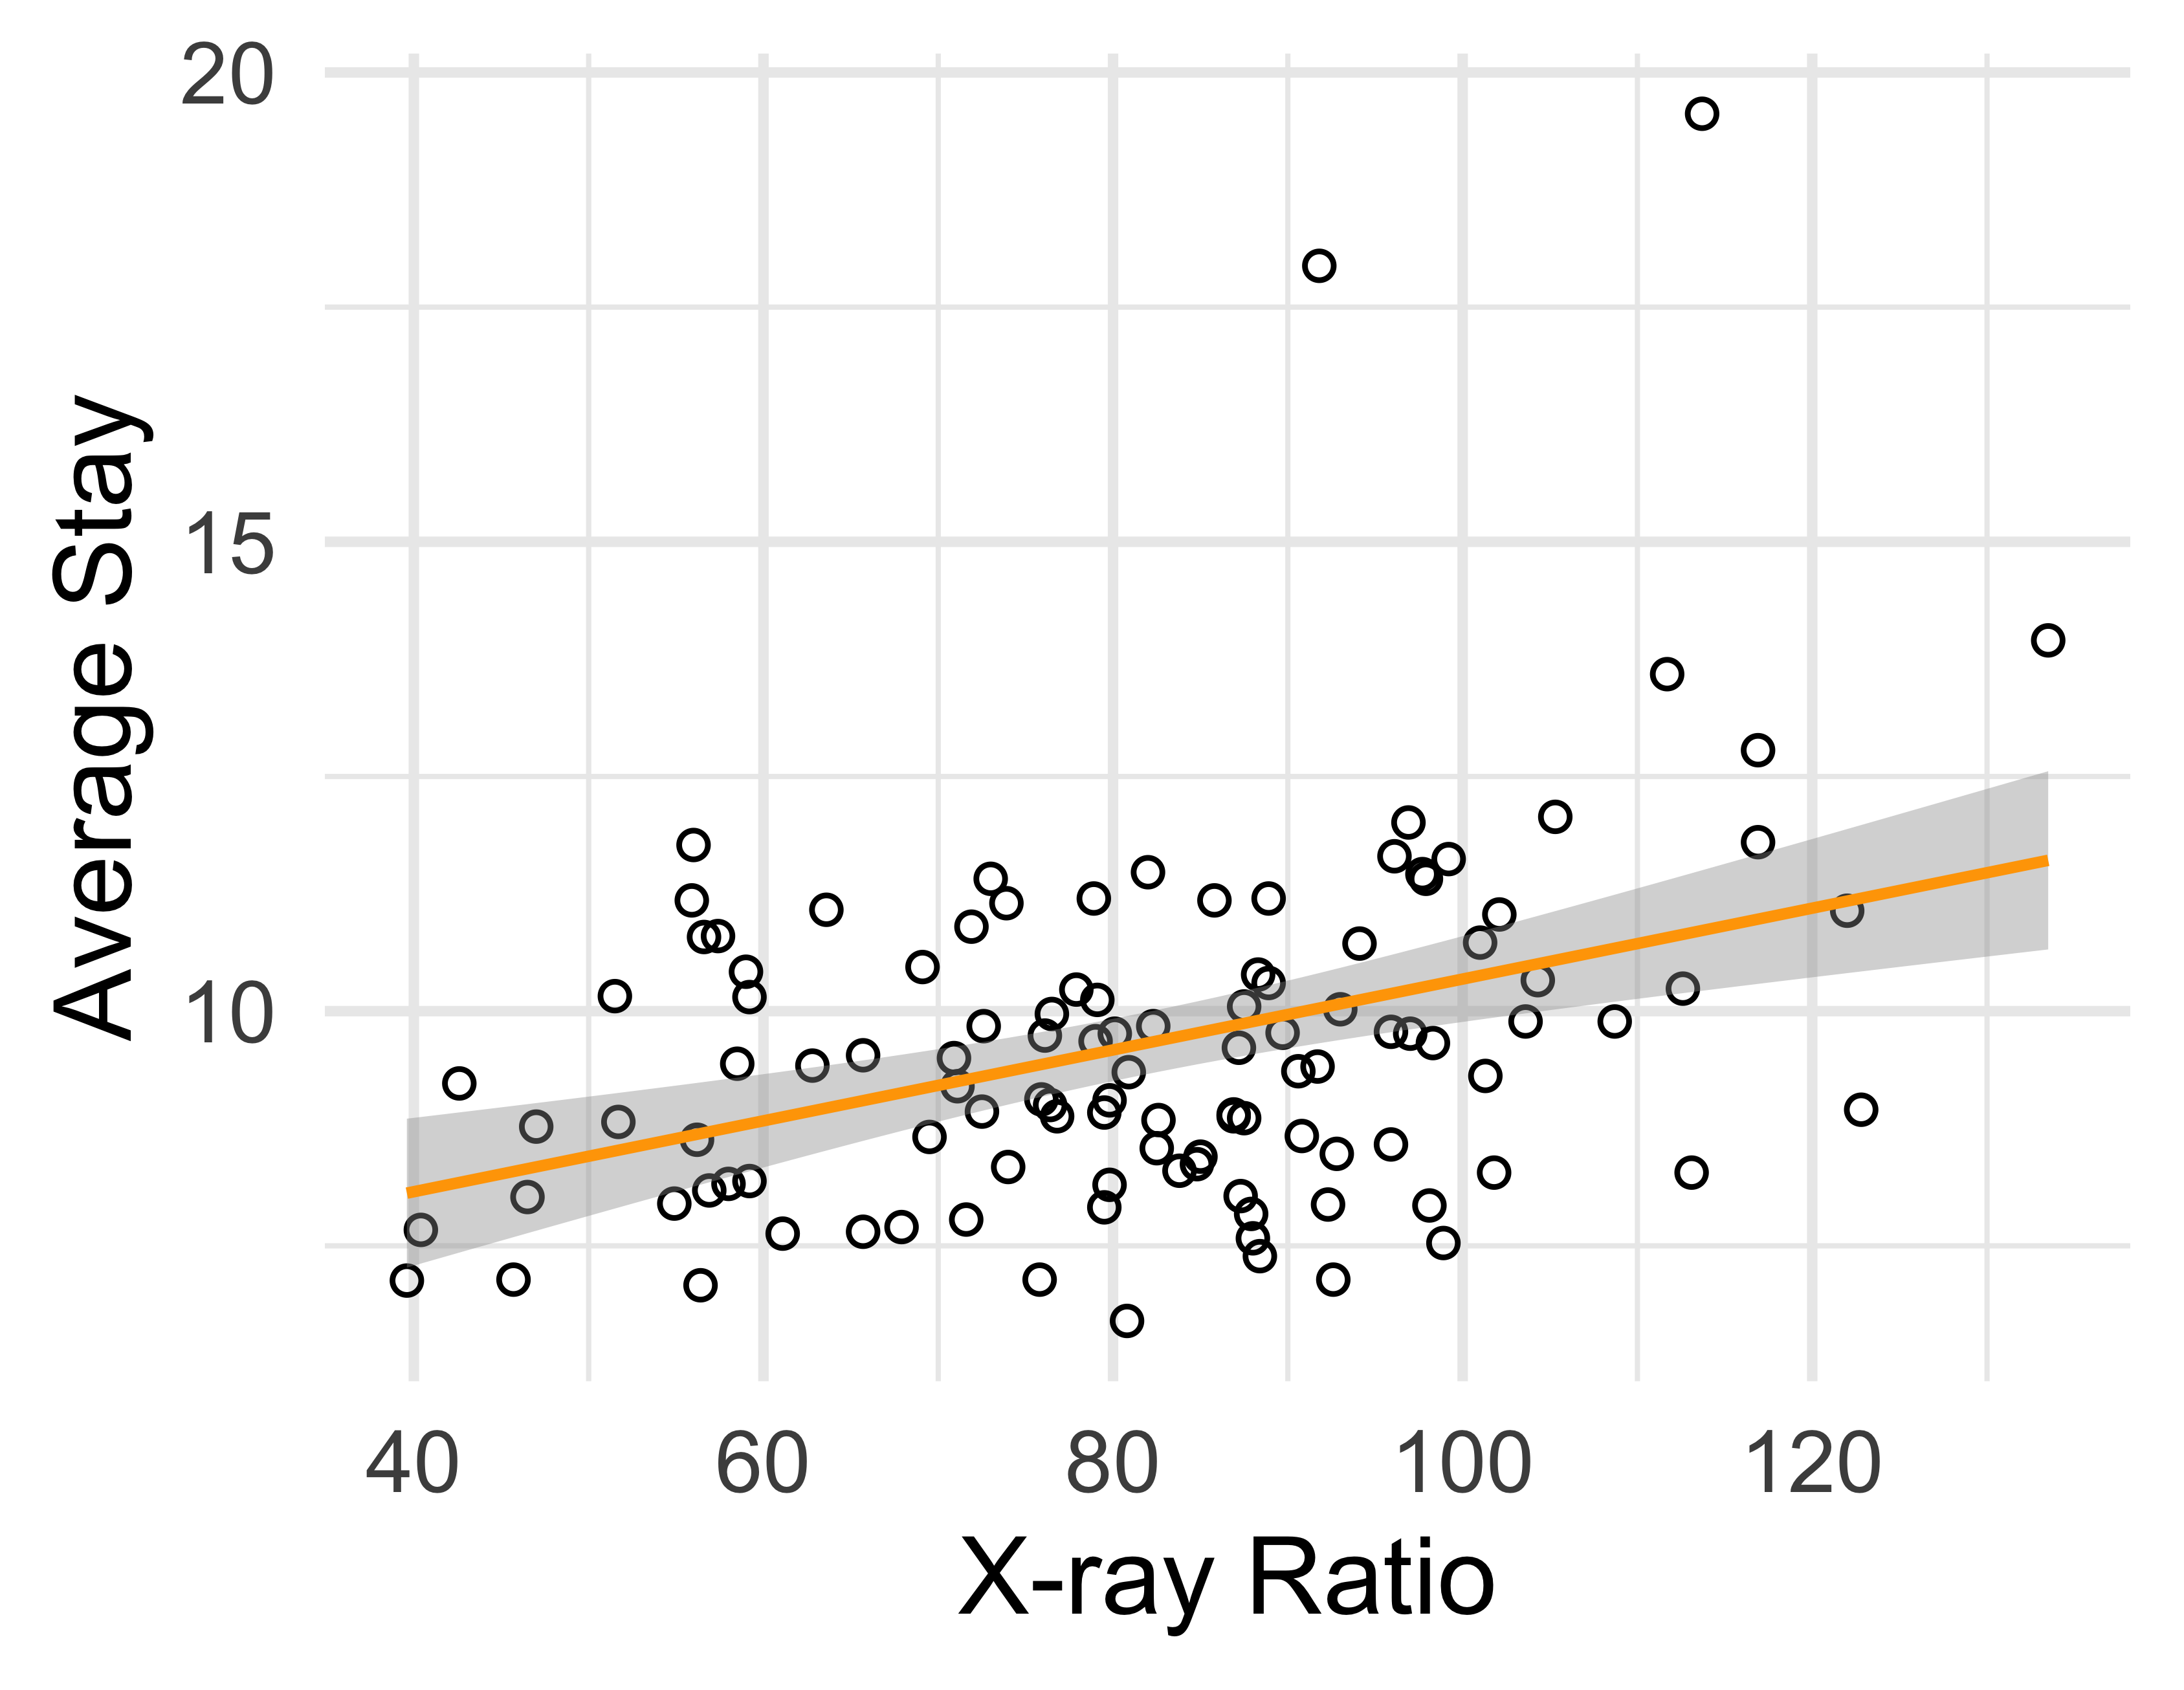
\includegraphics[width = 0.32\textwidth]{q02_lm3.png}
    \caption{Overlaying the estimated linear regression function for \texttt{Stay} against each of the three predictor variables.}
    \label{q02_fig02}
\end{figure}

\begin{itemize}
    \item[(a)] The loess smoothers have been overlayed each of their respective scatterplots in Figure \ref{q02_fig01}. We see that in each case the three 
    curves are not too volatile, so a linear regression model would not be completely out of the question. However, for \texttt{Risk} we see that the curve 
    begins to flatten out as we approach the end of the interval, and for \texttt{AFS} the curve begins to descend, both indications that the relationship is 
    nonlinear.
    For \texttt{Xray}, while the curve is ascending at both the beginning and the end, it is completely flat in the middle, another indication that the 
    relationship is nonlinear. 
    \item[(b)] For each predictor, the linear regression model was fit using \texttt{R} and overlayed on a scatterplot of \texttt{Stay} against that predictor. 
    While it is impossible for a linear model (or any model, for that matter) to account for the variance of the residuals, we can see that in all three cases,
    the slope of the regression line is positive. However, the lines are not steep, which indicates that, while there may be a positive linear relationship,
    it is not a strong one. Numerical details about each model, including the estimated coefficients, can be found in Table \ref{q02_tab01},
    which shows that all three slopes are positive but very small.
    \item[(c)] We use \texttt{R} to determine the estimated coefficients, mean squared error (MSE), and \(R^2\) value for each of the three models, all of 
    which can be found in Table \ref{q02_tab01}. 
    \begin{table}
        \centering
        \def\arraystretch{1.25}
        \begin{tabular}[ht]{ccccc} \toprule
            \(X\) & \(b_0\) & \(b_1\) & MSE & \(R^2\) \\ \midrule
            \texttt{Risk} & \(6.3368\) & \(0.7604\) & \(2.590837\) & \(0.2846\) \\
            \texttt{AFS} & \(7.71877\) & \(0.04471\) & \(3.163568\) & \(0.1264\) \\
            \texttt{Xray} & \(6.566373\) & \(0.037756\) & \(3.091558\) & \(0.1463\) \\ \bottomrule
        \end{tabular}
        \caption{Information about each of the three linear regression models for question 2.}
        \label{q02_tab01}
    \end{table}
    Recall that \(\mathrm{MSE} = \frac{1}{n}\|\mathbf{y} - b_0 \mathbf{1} - b_1 \mathbf{x}\|^2\), where \((\mathbf{x},\mathbf{y})\) are the vectors 
    corresponding 
    to the realized predictor and response variables, respectively. For a given model, a lower MSE (relative to the other models) indicates that the model is 
    a better fit than the others, since the residuals are smaller. In this case, we can see that the lowest MSE occurs when \texttt{Risk} is the predictor
    variable, which means that the residuals for the \texttt{Risk} model are generally lower than the other two. However, because the MSE for \texttt{Risk}
    is only marginally smaller than the other two, the residuals are not \textit{that} much smaller; Figure \ref{q02_fig02} serves as a gut check for this, 
    as the points spread out in all three plots, so it would not be obvious that \texttt{Risk} has the lowest MSE. We also see that \texttt{Risk} has the 
    highest \(R^2\) value; it is much higher relative to the other two models, but is still extremely low in its own right. That is, even though 
    \texttt{Risk} does a much better job than the other models explaining the variability in \texttt{Stay} than \texttt{AFS} or \texttt{Xray}, it still does 
    a pretty bad job overall. 
\end{itemize}

%' ============================================================================================================================================================
\section{Question 3} \noindent
For reference, the coefficients for the estimated linear regression function \(\hat{Y} = b_0 + b_1 X\) are
given by \[b_1 = \frac{\sum_{i=1}^n (x_i - \bar{x})(y_i - \bar{y})}{\sum_{i=1}^n(x_i - \bar{x})^2} ~~~\text{and}~~~ b_0 = \bar{y} - b_1 \bar{x}.\] 
The two \textit{normal equations} are given by 
\[
    \sum_{i=1}^{n} \left( y_i - b_0 - b_1 x_i \right) = 0 ~~\text{and}~~~ \sum_{i=1}^{n} x_i \left( y_i - b_0 - b_1 x_i \right) = 0
\]
We also note three useful manipulations:
\(\sum x_i = n \bar{x}\), \(\sum y_i = n \bar{y}\), and \(\bar{y} = b_0 + b_1 \bar{x}\).
The first two come from manipulating the definition of \(\bar{x}\) and \(\bar{y}\), respectively, and the third comes from manipulating the 
definition of \(b_0\).
\begin{itemize}
    \item[(a)] This is an immediate result of the first normal equation: 
    \[
        0 = \sum_{i=1}^{n} \left( y_i - b_0 - b_1 x_i \right) = \sum_{i=1}^n e_i.
    \]
    \item[(b)] This can be show directly:
    \[
        \sum_{i=1}^n \hat{y}_i = \sum_{i=1}^n \left( b_0 + b_1 x_i \right) = b_0 \sum_{i=1}^n 1 + b_1 \sum_{i=1}^n x_i
        = n b_0 + n b_1 \bar{x} = n(b_0 + b_1 \bar{x}) = n \bar{y} = \sum_{i=1}^n y_i.
    \]
    \item[(c)] This is an immediate result of the second normal equation:
    \[
        0 = \sum_{i=1}^{n} x_i \left( y_i - b_0 - b_1 x_i \right) = \sum_{i=1}^n x_i e_i.
    \]
    Let \(\mathbf{x} = (x_1,\ldots,x_n)^T\) be the vector of predictor observations and 
    \(\mathbf{e} = (e_1,\ldots,e_n)^T\) be the vector of residuals. This results implies that \(\langle\mathbf{x},\mathbf{e}\rangle = 0\), meaning
    \(\mathbf{x}\) and \(\mathbf{e}\) are \textit{orthogonal}.
    \item[(d)] Combining the results of parts (a) and (c), we have 
    \[
        \sum_{i=1}^n \hat{y}_i e_i = \sum_{i=1}^n \left( b_0 + b_1 x_i \right) e_i = b_0 \sum_{i=1}^n e_i + b_1 \sum_{i=1}^n x_i e_i
        = b_0 \cdot 0 + b_1 \cdot 0 = 0.
    \]
    If \(\hat{\mathbf{y}} = (\hat{y}_1,\ldots,\hat{y}_n)^T\) is the vector of fitted values, then \(\langle\hat{\mathbf{y}},\mathbf{e}\rangle=0\).
    \item[(e)] We want to show that \(\hat{y}_i = \bar{y}\) when \(x_i = \bar{x}\). This is actually an immediate result of the definition of \(b_0\)
    (the third manipulation), since 
    \(\hat{y}(\bar{x}) = b_0 + b_1 \bar{x} = \bar{y}\).
\end{itemize}

%' ============================================================================================================================================================
\section{Question 4} \noindent
Let \((X,Y)\sim p(x,y)\) with \(\mathbb{E}[X^2 + Y^2 < \infty]\).
\begin{itemize}
    \item[(a)] We want to find the value of \(c\) that minimizes \(\mathbb{E}\left[ (Y - c)^2\right]\). Expanding out the inside gives us 
    \[
        \mathbb{E} \left[ (Y - c)^2\right] = \mathbb{E} \left[Y^2 - 2cY + c^2\right]
        = \mathbb{E} \left[Y^2\right] + \mathbb{E} \left[-2cY\right] + \mathbb{E} \left[c^2\right] 
        = \mathbb{E} \left[Y^2\right] - 2c \mathbb{E} \left[Y\right] + c^2.
    \]
    Given that this is a function of \(c\), we will now differentiate this equation with respect to \(c\), i.e. 
    \[
        \frac{\mathrm{d}}{\mathrm{d}c} \Big( \mathbb{E} \left[Y^2\right] - 2c \mathbb{E} \left[Y\right] + c^2 \Big)
        = -2 \mathbb{E}[Y] + 2c \overset{\text{set}}{=} 0,
    \]
    and solving for \(c\) gives us \(c = \mathbb{E}[Y]\).
    \item[(b)] Using the subtle identity \(0 = \mathbb{E}[Y|X] - \mathbb{E}[Y|X]\), we have 
    \begin{align*}
        \big( Y - g(X)\big)^2 &= \big( Y - \mathbb{E}[Y|X] + \mathbb{E}[Y|X] - g(X)\big)^2 \\
        &= \Big( \big( Y - \mathbb{E}[Y|X] \big) + \big( \mathbb{E}[Y|X] - g(X) \big) \Big)^2 \\
        &= \big( Y - \mathbb{E}[Y|X] \big)^2 - 2 \big( Y - \mathbb{E}[Y|X] \big) \big( \mathbb{E}[Y|X] - g(X) \big)
        + \big( \mathbb{E}[Y|X] - g(X) \big)^2.
    \end{align*}
    Taking the expected value of this gives us 
    \begin{align*}
        \mathbb{E}&\left[ \big( Y - g(X)\big)^2 \right] \\
        &= \mathbb{E} \left[ 
            \big( Y - \mathbb{E}[Y|X] \big)^2 - 2 \big( Y - \mathbb{E}[Y|X] \big) \big( \mathbb{E}[Y|X] - g(X) \big)
            + \big( \mathbb{E}[Y|X] - g(X) \big)^2 \right] \\
        &= \mathbb{E}\left[ \big( Y - \mathbb{E}[Y|X] \big)^2 \right]
            + \mathbb{E}\left[ - 2 \big( Y - \mathbb{E}[Y|X] \big) \big( \mathbb{E}[Y|X] - g(X) \big) \right] 
            + \mathbb{E}\left[ \big( \mathbb{E}[Y|X] - g(X) \big)^2 \right] \\
        &= \mathbb{E}\left[ \big( Y - \mathbb{E}[Y|X] \big)^2 \right]
        -2 \big( \mathbb{E}[Y|X] - g(X) \big) \cdot \mathbb{E}\left[ Y - \mathbb{E}[Y|X]  \right]
        + \mathbb{E}\left[ \big( \mathbb{E}[Y|X] - g(X) \big)^2 \right].
    \end{align*}
    We now focus our attention on the middle term. Since we are taking the expecation with respect to \(X\),
    we have \(\mathbb{E}[Y] = \mathbb{E}\big[ \mathbb{E} [Y | X]\big]\), and so 
    \[\mathbb{E}\left[ Y - \mathbb{E}[Y|X]  \right] = \mathbb{E}[Y] - \mathbb{E}\big[ \mathbb{E} [Y | X]\big] = 
    \mathbb{E}\big[ \mathbb{E} [Y | X]\big] - \mathbb{E}\big[ \mathbb{E} [Y | X]\big] = 0.\]
    As a result, the middle term in the long expansion of \(\mathbb{E}\left[ \big( Y - g(X)\big)^2 \right]\) 
    dissapears, so we have 
    \[\mathbb{E}\left[ \big( Y - g(X)\big)^2 \right] = \mathbb{E}\left[ \big( Y - \mathbb{E}[Y|X] \big)^2 \right]
    + \mathbb{E}\left[ \big( \mathbb{E}[Y|X] - g(X) \big)^2 \right].\]
    Finally, because \((\cdot)^2 \ge 0\), we will have \(\big( \mathbb{E}[Y|X] - g(X) \big)^2 \ge 0\). Since the
    value of this random variable cannot be less than zero, we know its expected value cannot be negative either, i.e. 
    \(\mathbb{E}\left[ \big( \mathbb{E}[Y|X] - g(X) \big)^2 \right] \ge 0\). Therefore, we have 
    \[ \mathbb{E}\left[ \big( Y - g(X)\big)^2 \right] \ge \mathbb{E}\left[ \big( Y - \mathbb{E}[Y|X] \big)^2 \right]. \]
    That is, the minimum of the function \(\mathbb{E}\left[ \big( Y - g(X)\big)^2 \right]\) occurs when 
    \(g(X) = \mathbb{E}[Y|X]\), and since \(\mathbb{E}\left[ X^2 + Y^2 \right] < \infty\), this minimum is unique and
    well-defined. 
\end{itemize}

\end{document}